% Seccion consolidada del TFM sobre FP8. Incluir con % Seccion consolidada del TFM sobre FP8. Incluir con % Seccion consolidada del TFM sobre FP8. Incluir con % Seccion consolidada del TFM sobre FP8. Incluir con \input{docs/TFM/fp8.tex}.
% Requiere: \usepackage{graphicx,booktabs}. Ajusta rutas si compilas desde otro dir.
% Datos: results/hennessy-580/run_matmul_fp8/ultimo (job 20399). GB10 (sm_121), torch 2.9, triton 3.8.0.

\section{Reducción de precisión: FP8 en los tensor cores}
\label{sec:fp8}

La sección~\ref{sec:tma} concluye que el matmul denso en FP16 está pegado a
$\sim$90--100~TFLOP/s y que ese techo no lo pone la memoria sino la unidad MMA de
sm\_121: activar TMA no acelera. La única palanca para subir el techo de los tensor
cores en esta GPU es cambiar de precisión. Los tensor cores de Blackwell ejecutan FP8
al doble de throughput que FP16; se estudia si un kernel FP8 rompe la barrera y a qué
coste de precisión.

\subsection{Implementación}

Se añade un kernel (\texttt{src/CBKernels/triton/matmul\_fp8.py}) idéntico al baseline
salvo en el tipo de las entradas: A y B en \textbf{FP8 e4m3}
(\texttt{torch.float8\_e4m3fn}), \texttt{tl.dot} con acumulación en FP32 y salida FP16.
Mantener el resto igual (\emph{swizzling} L2, esquema de bloques) aísla el efecto de la
precisión. Se compara con el baseline FP16, con el propio kernel FP8 de Triton y con
\texttt{torch.\_scaled\_mm} (cuBLASLt), la ruta optimizada de NVIDIA. El error se
cuantifica como error relativo de Frobenius frente al resultado exacto en FP32.

\subsection{Resultados}

\begin{figure}[htbp]
  \centering
  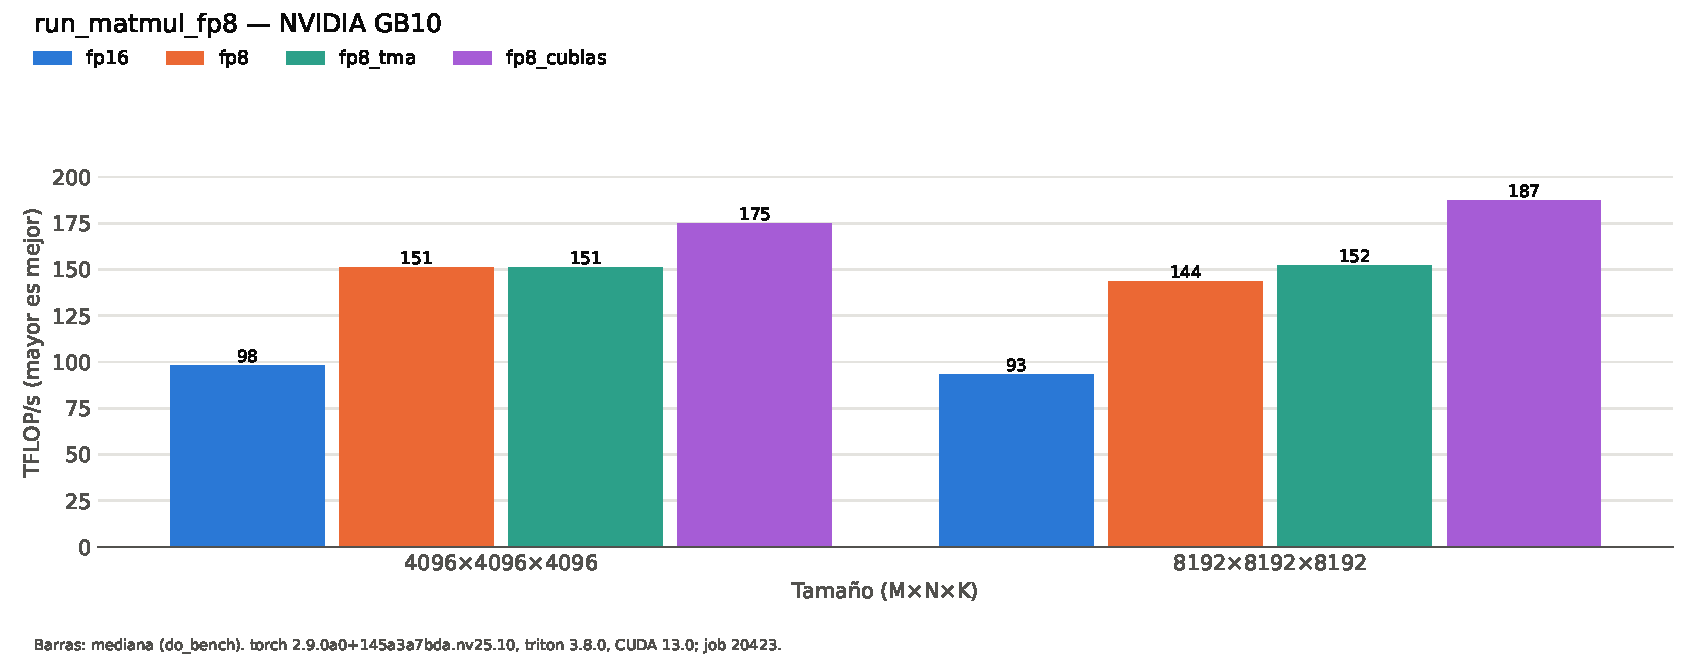
\includegraphics[width=\linewidth]{resultados/hennessy-580/figuras/run_matmul_fp8.pdf}
  \caption{Matmul en GB10: FP16 baseline vs FP8 (Triton) vs FP8 (cuBLASLt).}
  \label{fig:fp8}
\end{figure}

\input{resultados/hennessy-580/run_matmul_fp8.tex}

Resumen ($8192^3$): FP16 92{,}4; FP8 Triton 150{,}0 ($+62\,\%$); FP8 cuBLASLt
192{,}3~TFLOP/s. Error relativo FP8 $3{,}75\,\%$ frente a $0{,}02\,\%$ en FP16.

\subsection{Análisis}

\begin{enumerate}
  \item \textbf{FP8 rompe la barrera de los $\sim$100~TFLOP/s} que el matmul denso FP16
  no rebasaba (150~TFLOP/s en Triton, 192 en cuBLASLt), confirmando que el límite en
  FP16 era el cómputo (la MMA), no el transporte de datos.
  \item \textbf{El throughput viene de la instrucción MMA.} En FP8 el PTX emite
  \texttt{mma.sync.aligned.m16n8k32\dots e4m3.e4m3.f32}: el mismo tipo de MMA que en
  FP16 pero con $K=32$ (el doble que \texttt{m16n8k16}), origen del factor de mejora.
  \item \textbf{El coste es de precisión, no de estabilidad.} El error sube a
  $3{,}75\,\%$ (frente a $0{,}02\,\%$) por los $\sim$3 bits de mantisa de e4m3, pero es
  acotado e idéntico en Triton y cuBLASLt para las mismas entradas (límite del formato).
  \item \textbf{El kernel Triton deja margen frente a cuBLASLt} ($\approx 78\,\%$) y el
  $+62\,\%$ no alcanza el $2\times$ teórico: sobrecoste de \emph{pipelining} y
  \emph{autotuning}. Como en FP8 se mueve la mitad de bytes, el kernel puede acercarse a
  ser \emph{memory-bound}, y ahí el TMA por descriptores (§~\ref{sec:tma}) sí podría rendir.
\end{enumerate}

\subsection{Intento de cerrar el hueco: FP8 + TMA}

El kernel Triton FP8 alcanza $\sim$78--85\,\% de cuBLASLt. La hipótesis era que, al mover
FP8 la mitad de bytes, el kernel podría volverse \emph{memory-bound} y el TMA por
descriptores ---inútil en FP16 (§~\ref{sec:tma})--- sí ayudaría. Se implementa
\texttt{matmul\_fp8\_tma} (FP8 + \texttt{tl.make\_tensor\_descriptor}, autotuning ampliado).
El kernel emite TMA de verdad (verificado en PTX) pero solo gana \textbf{+1{,}5\,\%}
(150{,}5 vs 148{,}3~TFLOP/s en $8192^3$; cuBLASLt 182{,}3). La hipótesis es incorrecta:
FP8 tampoco está limitado por la memoria, y el \emph{autotuner} ni siquiera eligió bloques
grandes ni más \emph{stages}. \textbf{El hueco restante ($\sim$18\,\%) no está en los datos
ni en el tiling, sino en el \emph{scheduling}} de cuBLASLt (kernels persistentes,
especialización de warps), fuera del alcance del kernel de una onda por tile.

\subsection{Conclusión}

La reducción a FP8 e4m3 es la técnica que efectivamente sube el techo de los tensor
cores en GB10 ($+57$--$62\,\%$), a cambio de un error relativo acotado del $\sim$3{,}75\,\%,
coherente con que la MMA fuese el cuello en FP16. El kernel Triton llega a $\sim$83\,\% de
cuBLASLt y el hueco no se cierra con TMA (es \emph{scheduling}, no datos): requeriría un
kernel persistente, línea que se deja indicada. La vía con mayor recorrido para subir el
techo es la estructura dispersa 2:4 (§~\ref{sec:sparsity}), única que puede acercarse a la
cifra de catálogo.
.
% Requiere: \usepackage{graphicx,booktabs}. Ajusta rutas si compilas desde otro dir.
% Datos: results/hennessy-580/run_matmul_fp8/ultimo (job 20399). GB10 (sm_121), torch 2.9, triton 3.8.0.

\section{Reducción de precisión: FP8 en los tensor cores}
\label{sec:fp8}

La sección~\ref{sec:tma} concluye que el matmul denso en FP16 está pegado a
$\sim$90--100~TFLOP/s y que ese techo no lo pone la memoria sino la unidad MMA de
sm\_121: activar TMA no acelera. La única palanca para subir el techo de los tensor
cores en esta GPU es cambiar de precisión. Los tensor cores de Blackwell ejecutan FP8
al doble de throughput que FP16; se estudia si un kernel FP8 rompe la barrera y a qué
coste de precisión.

\subsection{Implementación}

Se añade un kernel (\texttt{src/CBKernels/triton/matmul\_fp8.py}) idéntico al baseline
salvo en el tipo de las entradas: A y B en \textbf{FP8 e4m3}
(\texttt{torch.float8\_e4m3fn}), \texttt{tl.dot} con acumulación en FP32 y salida FP16.
Mantener el resto igual (\emph{swizzling} L2, esquema de bloques) aísla el efecto de la
precisión. Se compara con el baseline FP16, con el propio kernel FP8 de Triton y con
\texttt{torch.\_scaled\_mm} (cuBLASLt), la ruta optimizada de NVIDIA. El error se
cuantifica como error relativo de Frobenius frente al resultado exacto en FP32.

\subsection{Resultados}

\begin{figure}[htbp]
  \centering
  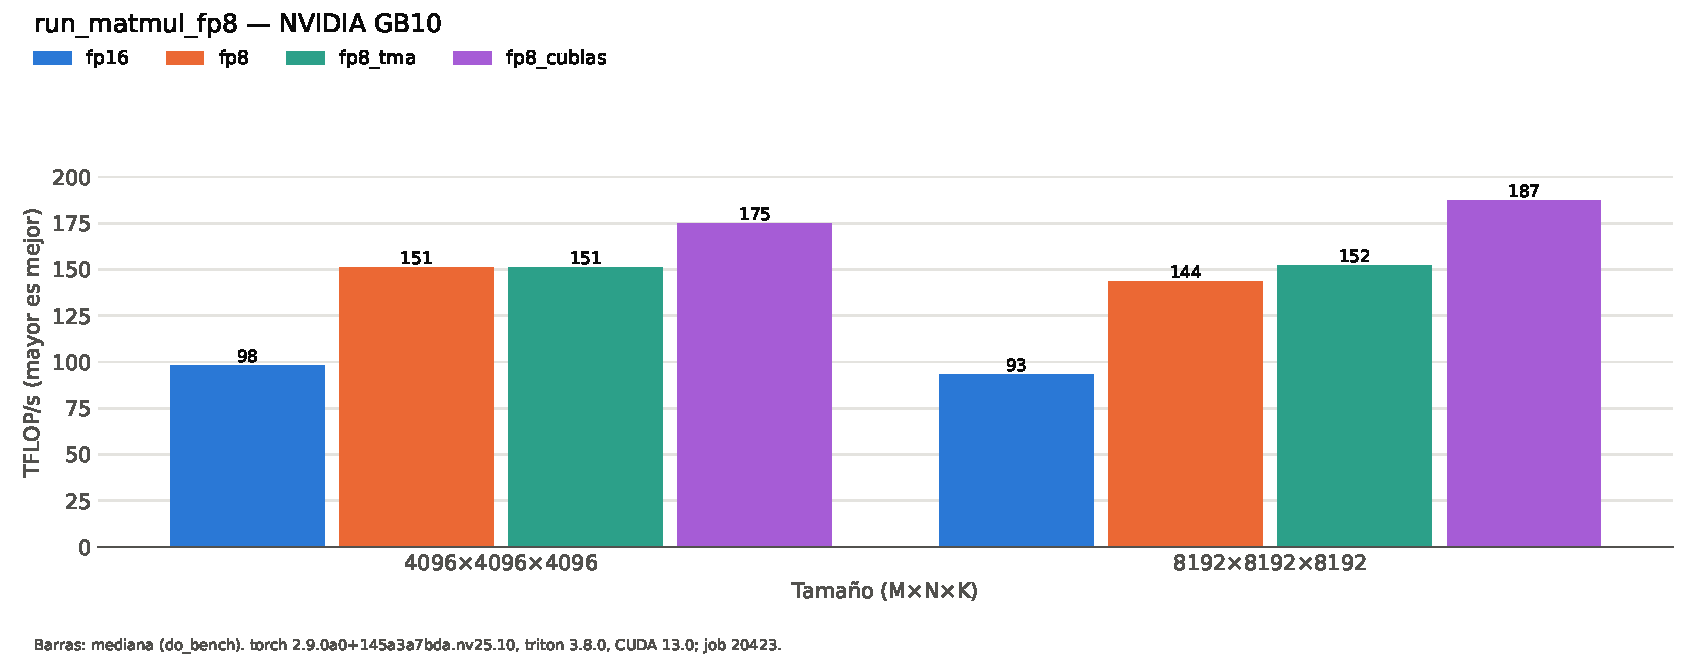
\includegraphics[width=\linewidth]{resultados/hennessy-580/figuras/run_matmul_fp8.pdf}
  \caption{Matmul en GB10: FP16 baseline vs FP8 (Triton) vs FP8 (cuBLASLt).}
  \label{fig:fp8}
\end{figure}

% Requiere \usepackage{booktabs}
\begin{table}[htbp]
  \centering\small
  \begin{tabular}{lrrrlllllllrrrrrrl}
    \toprule
    variante & M & N & K & BLOCK\_SIZE\_M & BLOCK\_SIZE\_N & BLOCK\_SIZE\_K & GROUP\_SIZE\_M & num\_warps & num\_stages & carga & error\_rel & ms & ms\_p20 & ms\_p80 & tflops & gbs & mma \\
    \midrule
    fp16 & 4096 & 4096 & 4096 & 128 & 128 & 32 & 8 & 4 & 4 & cp.async & 0.00021 & 1.4033 & 1.3978 & 1.5971 & 97.94 & 71.7 & mma.sync.aligned.m16n8k16.row.col.f32.f16.f16.f32 \\
    fp8 & 4096 & 4096 & 4096 & 256 & 128 & 128 & 8 & 8 & 3 & cp.async & 0.03752 & 0.9103 & 0.9073 & 0.9185 & 150.98 & 73.7 & mma.sync.aligned.m16n8k32.row.col.f32.e4m3.e4m3.f32 \\
    fp8\_tma & 4096 & 4096 & 4096 & 128 & 128 & 64 & 8 & 4 & 4 & TMA & 0.03752 & 0.9093 & 0.9073 & 0.9155 & 151.15 & 73.8 & mma.sync.aligned.m16n8k32.row.col.f32.e4m3.e4m3.f32 \\
    fp8\_cublas & 4096 & 4096 & 4096 &  &  &  &  &  &  & cublasLt & 0.03752 & 0.7854 & 0.7803 & 0.7967 & 175 & 85.4 & cublasLt \\
    fp16 & 8192 & 8192 & 8192 & 128 & 256 & 64 & 8 & 8 & 3 & cp.async & 0.00021 & 11.8026 & 11.7821 & 12.3607 & 93.16 & 34.1 & mma.sync.aligned.m16n8k16.row.col.f32.f16.f16.f32 \\
    fp8 & 8192 & 8192 & 8192 & 256 & 128 & 128 & 8 & 8 & 3 & cp.async & 0.03755 & 7.6595 & 7.6275 & 7.9587 & 143.55 & 35 & mma.sync.aligned.m16n8k32.row.col.f32.e4m3.e4m3.f32 \\
    fp8\_tma & 8192 & 8192 & 8192 & 128 & 256 & 128 & 8 & 8 & 3 & TMA & 0.03755 & 7.2253 & 7.2083 & 7.6075 & 152.18 & 37.2 & mma.sync.aligned.m16n8k32.row.col.f32.e4m3.e4m3.f32 \\
    fp8\_cublas & 8192 & 8192 & 8192 &  &  &  &  &  &  & cublasLt & 0.03755 & 5.8716 & 5.8011 & 5.9836 & 187.26 & 45.7 & cublasLt \\
    \bottomrule
  \end{tabular}
  \caption{run\_matmul\_fp8: NVIDIA GB10 (sm\_121), torch 2.9.0a0+145a3a7bda.nv25.10, triton 3.8.0, CUDA 13.0; job 20423, 2026-09-30T14:15:01. Mediana de triton.testing.do\_bench.}
  \label{tab:run-matmul-fp8}
\end{table}


Resumen ($8192^3$): FP16 92{,}4; FP8 Triton 150{,}0 ($+62\,\%$); FP8 cuBLASLt
192{,}3~TFLOP/s. Error relativo FP8 $3{,}75\,\%$ frente a $0{,}02\,\%$ en FP16.

\subsection{Análisis}

\begin{enumerate}
  \item \textbf{FP8 rompe la barrera de los $\sim$100~TFLOP/s} que el matmul denso FP16
  no rebasaba (150~TFLOP/s en Triton, 192 en cuBLASLt), confirmando que el límite en
  FP16 era el cómputo (la MMA), no el transporte de datos.
  \item \textbf{El throughput viene de la instrucción MMA.} En FP8 el PTX emite
  \texttt{mma.sync.aligned.m16n8k32\dots e4m3.e4m3.f32}: el mismo tipo de MMA que en
  FP16 pero con $K=32$ (el doble que \texttt{m16n8k16}), origen del factor de mejora.
  \item \textbf{El coste es de precisión, no de estabilidad.} El error sube a
  $3{,}75\,\%$ (frente a $0{,}02\,\%$) por los $\sim$3 bits de mantisa de e4m3, pero es
  acotado e idéntico en Triton y cuBLASLt para las mismas entradas (límite del formato).
  \item \textbf{El kernel Triton deja margen frente a cuBLASLt} ($\approx 78\,\%$) y el
  $+62\,\%$ no alcanza el $2\times$ teórico: sobrecoste de \emph{pipelining} y
  \emph{autotuning}. Como en FP8 se mueve la mitad de bytes, el kernel puede acercarse a
  ser \emph{memory-bound}, y ahí el TMA por descriptores (§~\ref{sec:tma}) sí podría rendir.
\end{enumerate}

\subsection{Intento de cerrar el hueco: FP8 + TMA}

El kernel Triton FP8 alcanza $\sim$78--85\,\% de cuBLASLt. La hipótesis era que, al mover
FP8 la mitad de bytes, el kernel podría volverse \emph{memory-bound} y el TMA por
descriptores ---inútil en FP16 (§~\ref{sec:tma})--- sí ayudaría. Se implementa
\texttt{matmul\_fp8\_tma} (FP8 + \texttt{tl.make\_tensor\_descriptor}, autotuning ampliado).
El kernel emite TMA de verdad (verificado en PTX) pero solo gana \textbf{+1{,}5\,\%}
(150{,}5 vs 148{,}3~TFLOP/s en $8192^3$; cuBLASLt 182{,}3). La hipótesis es incorrecta:
FP8 tampoco está limitado por la memoria, y el \emph{autotuner} ni siquiera eligió bloques
grandes ni más \emph{stages}. \textbf{El hueco restante ($\sim$18\,\%) no está en los datos
ni en el tiling, sino en el \emph{scheduling}} de cuBLASLt (kernels persistentes,
especialización de warps), fuera del alcance del kernel de una onda por tile.

\subsection{Conclusión}

La reducción a FP8 e4m3 es la técnica que efectivamente sube el techo de los tensor
cores en GB10 ($+57$--$62\,\%$), a cambio de un error relativo acotado del $\sim$3{,}75\,\%,
coherente con que la MMA fuese el cuello en FP16. El kernel Triton llega a $\sim$83\,\% de
cuBLASLt y el hueco no se cierra con TMA (es \emph{scheduling}, no datos): requeriría un
kernel persistente, línea que se deja indicada. La vía con mayor recorrido para subir el
techo es la estructura dispersa 2:4 (§~\ref{sec:sparsity}), única que puede acercarse a la
cifra de catálogo.
.
% Requiere: \usepackage{graphicx,booktabs}. Ajusta rutas si compilas desde otro dir.
% Datos: results/hennessy-580/run_matmul_fp8/ultimo (job 20399). GB10 (sm_121), torch 2.9, triton 3.8.0.

\section{Reducción de precisión: FP8 en los tensor cores}
\label{sec:fp8}

La sección~\ref{sec:tma} concluye que el matmul denso en FP16 está pegado a
$\sim$90--100~TFLOP/s y que ese techo no lo pone la memoria sino la unidad MMA de
sm\_121: activar TMA no acelera. La única palanca para subir el techo de los tensor
cores en esta GPU es cambiar de precisión. Los tensor cores de Blackwell ejecutan FP8
al doble de throughput que FP16; se estudia si un kernel FP8 rompe la barrera y a qué
coste de precisión.

\subsection{Implementación}

Se añade un kernel (\texttt{src/CBKernels/triton/matmul\_fp8.py}) idéntico al baseline
salvo en el tipo de las entradas: A y B en \textbf{FP8 e4m3}
(\texttt{torch.float8\_e4m3fn}), \texttt{tl.dot} con acumulación en FP32 y salida FP16.
Mantener el resto igual (\emph{swizzling} L2, esquema de bloques) aísla el efecto de la
precisión. Se compara con el baseline FP16, con el propio kernel FP8 de Triton y con
\texttt{torch.\_scaled\_mm} (cuBLASLt), la ruta optimizada de NVIDIA. El error se
cuantifica como error relativo de Frobenius frente al resultado exacto en FP32.

\subsection{Resultados}

\begin{figure}[htbp]
  \centering
  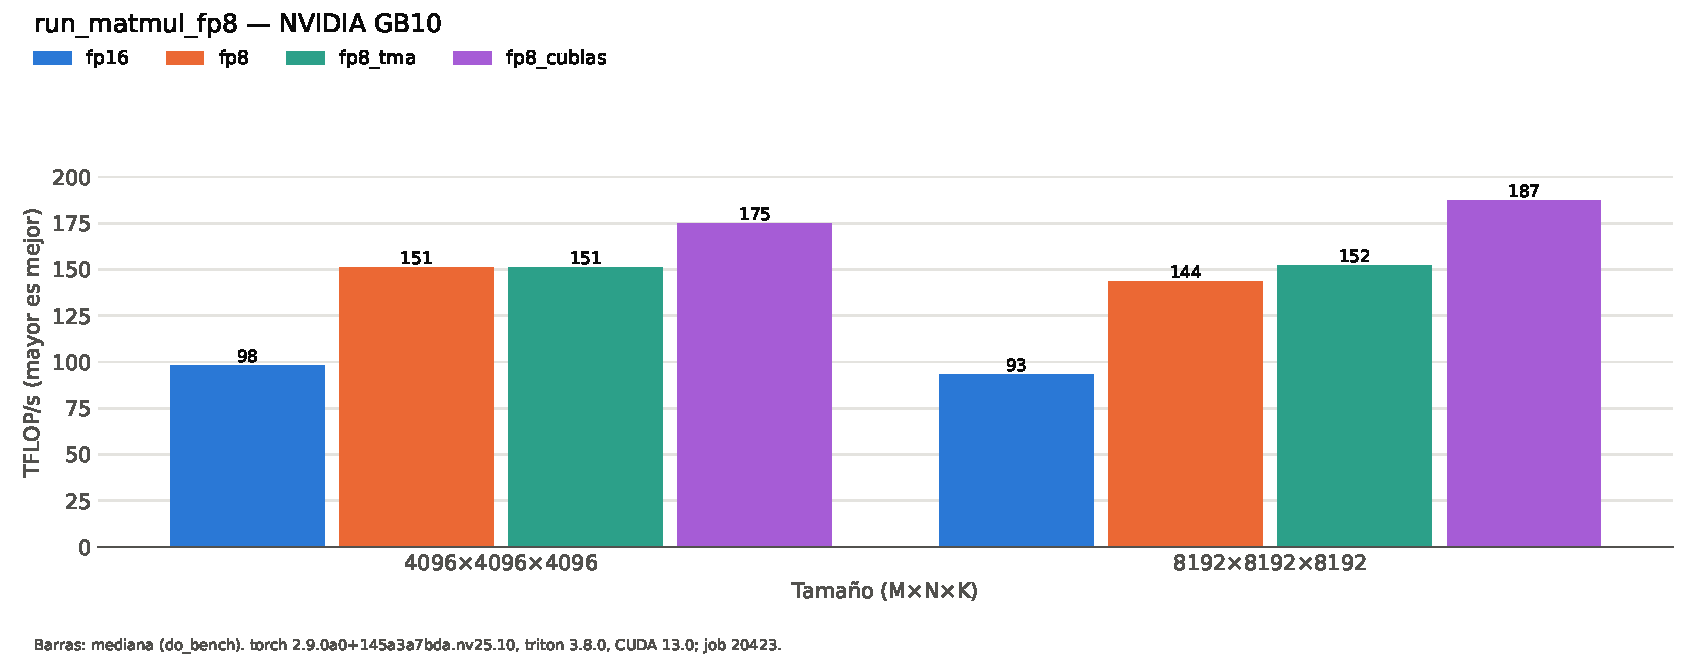
\includegraphics[width=\linewidth]{resultados/hennessy-580/figuras/run_matmul_fp8.pdf}
  \caption{Matmul en GB10: FP16 baseline vs FP8 (Triton) vs FP8 (cuBLASLt).}
  \label{fig:fp8}
\end{figure}

% Requiere \usepackage{booktabs}
\begin{table}[htbp]
  \centering\small
  \begin{tabular}{lrrrlllllllrrrrrrl}
    \toprule
    variante & M & N & K & BLOCK\_SIZE\_M & BLOCK\_SIZE\_N & BLOCK\_SIZE\_K & GROUP\_SIZE\_M & num\_warps & num\_stages & carga & error\_rel & ms & ms\_p20 & ms\_p80 & tflops & gbs & mma \\
    \midrule
    fp16 & 4096 & 4096 & 4096 & 128 & 128 & 32 & 8 & 4 & 4 & cp.async & 0.00021 & 1.4033 & 1.3978 & 1.5971 & 97.94 & 71.7 & mma.sync.aligned.m16n8k16.row.col.f32.f16.f16.f32 \\
    fp8 & 4096 & 4096 & 4096 & 256 & 128 & 128 & 8 & 8 & 3 & cp.async & 0.03752 & 0.9103 & 0.9073 & 0.9185 & 150.98 & 73.7 & mma.sync.aligned.m16n8k32.row.col.f32.e4m3.e4m3.f32 \\
    fp8\_tma & 4096 & 4096 & 4096 & 128 & 128 & 64 & 8 & 4 & 4 & TMA & 0.03752 & 0.9093 & 0.9073 & 0.9155 & 151.15 & 73.8 & mma.sync.aligned.m16n8k32.row.col.f32.e4m3.e4m3.f32 \\
    fp8\_cublas & 4096 & 4096 & 4096 &  &  &  &  &  &  & cublasLt & 0.03752 & 0.7854 & 0.7803 & 0.7967 & 175 & 85.4 & cublasLt \\
    fp16 & 8192 & 8192 & 8192 & 128 & 256 & 64 & 8 & 8 & 3 & cp.async & 0.00021 & 11.8026 & 11.7821 & 12.3607 & 93.16 & 34.1 & mma.sync.aligned.m16n8k16.row.col.f32.f16.f16.f32 \\
    fp8 & 8192 & 8192 & 8192 & 256 & 128 & 128 & 8 & 8 & 3 & cp.async & 0.03755 & 7.6595 & 7.6275 & 7.9587 & 143.55 & 35 & mma.sync.aligned.m16n8k32.row.col.f32.e4m3.e4m3.f32 \\
    fp8\_tma & 8192 & 8192 & 8192 & 128 & 256 & 128 & 8 & 8 & 3 & TMA & 0.03755 & 7.2253 & 7.2083 & 7.6075 & 152.18 & 37.2 & mma.sync.aligned.m16n8k32.row.col.f32.e4m3.e4m3.f32 \\
    fp8\_cublas & 8192 & 8192 & 8192 &  &  &  &  &  &  & cublasLt & 0.03755 & 5.8716 & 5.8011 & 5.9836 & 187.26 & 45.7 & cublasLt \\
    \bottomrule
  \end{tabular}
  \caption{run\_matmul\_fp8: NVIDIA GB10 (sm\_121), torch 2.9.0a0+145a3a7bda.nv25.10, triton 3.8.0, CUDA 13.0; job 20423, 2026-09-30T14:15:01. Mediana de triton.testing.do\_bench.}
  \label{tab:run-matmul-fp8}
\end{table}


Resumen ($8192^3$): FP16 92{,}4; FP8 Triton 150{,}0 ($+62\,\%$); FP8 cuBLASLt
192{,}3~TFLOP/s. Error relativo FP8 $3{,}75\,\%$ frente a $0{,}02\,\%$ en FP16.

\subsection{Análisis}

\begin{enumerate}
  \item \textbf{FP8 rompe la barrera de los $\sim$100~TFLOP/s} que el matmul denso FP16
  no rebasaba (150~TFLOP/s en Triton, 192 en cuBLASLt), confirmando que el límite en
  FP16 era el cómputo (la MMA), no el transporte de datos.
  \item \textbf{El throughput viene de la instrucción MMA.} En FP8 el PTX emite
  \texttt{mma.sync.aligned.m16n8k32\dots e4m3.e4m3.f32}: el mismo tipo de MMA que en
  FP16 pero con $K=32$ (el doble que \texttt{m16n8k16}), origen del factor de mejora.
  \item \textbf{El coste es de precisión, no de estabilidad.} El error sube a
  $3{,}75\,\%$ (frente a $0{,}02\,\%$) por los $\sim$3 bits de mantisa de e4m3, pero es
  acotado e idéntico en Triton y cuBLASLt para las mismas entradas (límite del formato).
  \item \textbf{El kernel Triton deja margen frente a cuBLASLt} ($\approx 78\,\%$) y el
  $+62\,\%$ no alcanza el $2\times$ teórico: sobrecoste de \emph{pipelining} y
  \emph{autotuning}. Como en FP8 se mueve la mitad de bytes, el kernel puede acercarse a
  ser \emph{memory-bound}, y ahí el TMA por descriptores (§~\ref{sec:tma}) sí podría rendir.
\end{enumerate}

\subsection{Intento de cerrar el hueco: FP8 + TMA}

El kernel Triton FP8 alcanza $\sim$78--85\,\% de cuBLASLt. La hipótesis era que, al mover
FP8 la mitad de bytes, el kernel podría volverse \emph{memory-bound} y el TMA por
descriptores ---inútil en FP16 (§~\ref{sec:tma})--- sí ayudaría. Se implementa
\texttt{matmul\_fp8\_tma} (FP8 + \texttt{tl.make\_tensor\_descriptor}, autotuning ampliado).
El kernel emite TMA de verdad (verificado en PTX) pero solo gana \textbf{+1{,}5\,\%}
(150{,}5 vs 148{,}3~TFLOP/s en $8192^3$; cuBLASLt 182{,}3). La hipótesis es incorrecta:
FP8 tampoco está limitado por la memoria, y el \emph{autotuner} ni siquiera eligió bloques
grandes ni más \emph{stages}. \textbf{El hueco restante ($\sim$18\,\%) no está en los datos
ni en el tiling, sino en el \emph{scheduling}} de cuBLASLt (kernels persistentes,
especialización de warps), fuera del alcance del kernel de una onda por tile.

\subsection{Conclusión}

La reducción a FP8 e4m3 es la técnica que efectivamente sube el techo de los tensor
cores en GB10 ($+57$--$62\,\%$), a cambio de un error relativo acotado del $\sim$3{,}75\,\%,
coherente con que la MMA fuese el cuello en FP16. El kernel Triton llega a $\sim$83\,\% de
cuBLASLt y el hueco no se cierra con TMA (es \emph{scheduling}, no datos): requeriría un
kernel persistente, línea que se deja indicada. La vía con mayor recorrido para subir el
techo es la estructura dispersa 2:4 (§~\ref{sec:sparsity}), única que puede acercarse a la
cifra de catálogo.
.
% Requiere: \usepackage{graphicx,booktabs}. Ajusta rutas si compilas desde otro dir.
% Datos: results/hennessy-580/run_matmul_fp8/ultimo (job 20399). GB10 (sm_121), torch 2.9, triton 3.8.0.

\section{Reducción de precisión: FP8 en los tensor cores}
\label{sec:fp8}

La sección~\ref{sec:tma} concluye que el matmul denso en FP16 está pegado a
$\sim$90--100~TFLOP/s y que ese techo no lo pone la memoria sino la unidad MMA de
sm\_121: activar TMA no acelera. La única palanca para subir el techo de los tensor
cores en esta GPU es cambiar de precisión. Los tensor cores de Blackwell ejecutan FP8
al doble de throughput que FP16; se estudia si un kernel FP8 rompe la barrera y a qué
coste de precisión.

\subsection{Implementación}

Se añade un kernel (\texttt{src/CBKernels/triton/matmul\_fp8.py}) idéntico al baseline
salvo en el tipo de las entradas: A y B en \textbf{FP8 e4m3}
(\texttt{torch.float8\_e4m3fn}), \texttt{tl.dot} con acumulación en FP32 y salida FP16.
Mantener el resto igual (\emph{swizzling} L2, esquema de bloques) aísla el efecto de la
precisión. Se compara con el baseline FP16, con el propio kernel FP8 de Triton y con
\texttt{torch.\_scaled\_mm} (cuBLASLt), la ruta optimizada de NVIDIA. El error se
cuantifica como error relativo de Frobenius frente al resultado exacto en FP32.

\subsection{Resultados}

\begin{figure}[htbp]
  \centering
  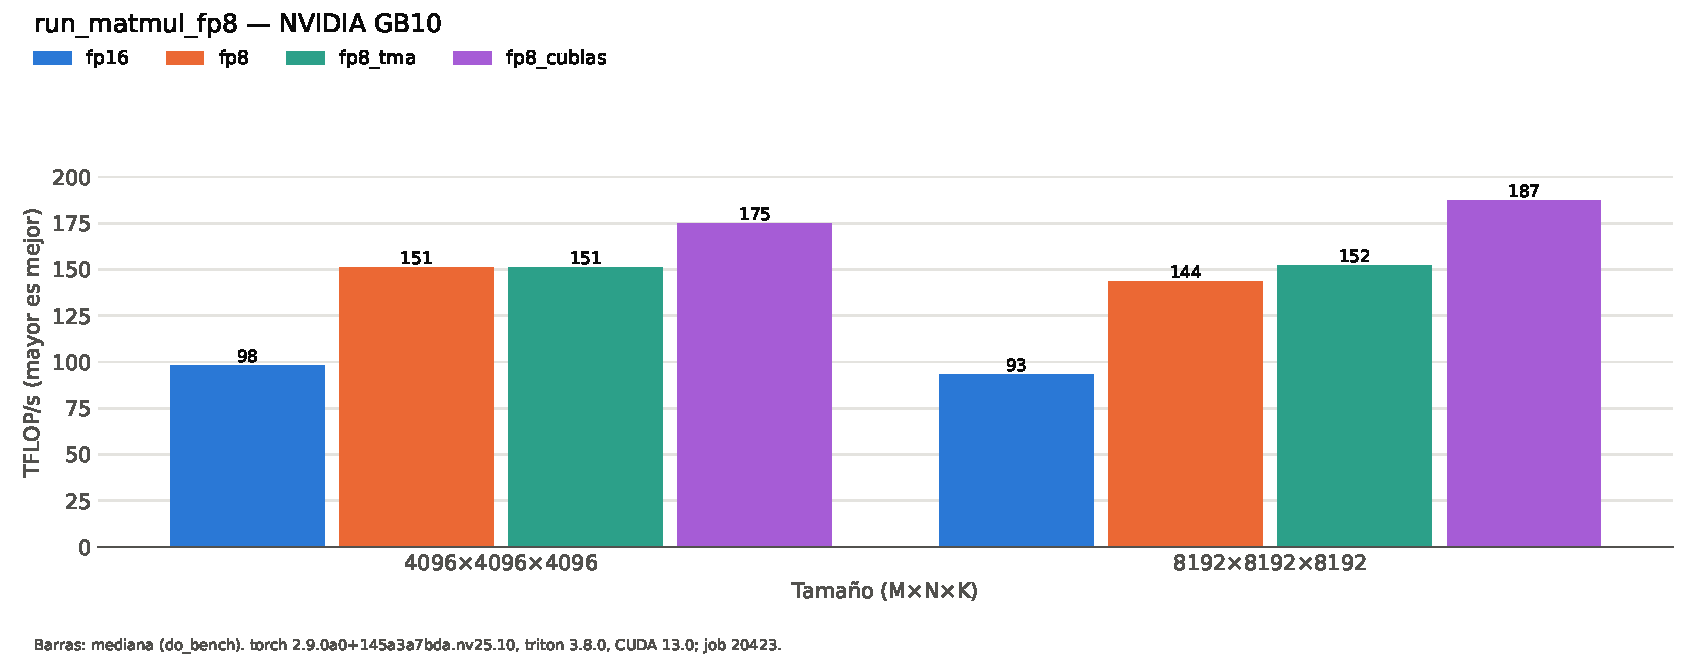
\includegraphics[width=\linewidth]{resultados/hennessy-580/figuras/run_matmul_fp8.pdf}
  \caption{Matmul en GB10: FP16 baseline vs FP8 (Triton) vs FP8 (cuBLASLt).}
  \label{fig:fp8}
\end{figure}

% Requiere \usepackage{booktabs}
\begin{table}[htbp]
  \centering\small
  \begin{tabular}{lrrrlllllllrrrrrrl}
    \toprule
    variante & M & N & K & BLOCK\_SIZE\_M & BLOCK\_SIZE\_N & BLOCK\_SIZE\_K & GROUP\_SIZE\_M & num\_warps & num\_stages & carga & error\_rel & ms & ms\_p20 & ms\_p80 & tflops & gbs & mma \\
    \midrule
    fp16 & 4096 & 4096 & 4096 & 128 & 128 & 32 & 8 & 4 & 4 & cp.async & 0.00021 & 1.4033 & 1.3978 & 1.5971 & 97.94 & 71.7 & mma.sync.aligned.m16n8k16.row.col.f32.f16.f16.f32 \\
    fp8 & 4096 & 4096 & 4096 & 256 & 128 & 128 & 8 & 8 & 3 & cp.async & 0.03752 & 0.9103 & 0.9073 & 0.9185 & 150.98 & 73.7 & mma.sync.aligned.m16n8k32.row.col.f32.e4m3.e4m3.f32 \\
    fp8\_tma & 4096 & 4096 & 4096 & 128 & 128 & 64 & 8 & 4 & 4 & TMA & 0.03752 & 0.9093 & 0.9073 & 0.9155 & 151.15 & 73.8 & mma.sync.aligned.m16n8k32.row.col.f32.e4m3.e4m3.f32 \\
    fp8\_cublas & 4096 & 4096 & 4096 &  &  &  &  &  &  & cublasLt & 0.03752 & 0.7854 & 0.7803 & 0.7967 & 175 & 85.4 & cublasLt \\
    fp16 & 8192 & 8192 & 8192 & 128 & 256 & 64 & 8 & 8 & 3 & cp.async & 0.00021 & 11.8026 & 11.7821 & 12.3607 & 93.16 & 34.1 & mma.sync.aligned.m16n8k16.row.col.f32.f16.f16.f32 \\
    fp8 & 8192 & 8192 & 8192 & 256 & 128 & 128 & 8 & 8 & 3 & cp.async & 0.03755 & 7.6595 & 7.6275 & 7.9587 & 143.55 & 35 & mma.sync.aligned.m16n8k32.row.col.f32.e4m3.e4m3.f32 \\
    fp8\_tma & 8192 & 8192 & 8192 & 128 & 256 & 128 & 8 & 8 & 3 & TMA & 0.03755 & 7.2253 & 7.2083 & 7.6075 & 152.18 & 37.2 & mma.sync.aligned.m16n8k32.row.col.f32.e4m3.e4m3.f32 \\
    fp8\_cublas & 8192 & 8192 & 8192 &  &  &  &  &  &  & cublasLt & 0.03755 & 5.8716 & 5.8011 & 5.9836 & 187.26 & 45.7 & cublasLt \\
    \bottomrule
  \end{tabular}
  \caption{run\_matmul\_fp8: NVIDIA GB10 (sm\_121), torch 2.9.0a0+145a3a7bda.nv25.10, triton 3.8.0, CUDA 13.0; job 20423, 2026-09-30T14:15:01. Mediana de triton.testing.do\_bench.}
  \label{tab:run-matmul-fp8}
\end{table}


Resumen ($8192^3$): FP16 92{,}4; FP8 Triton 150{,}0 ($+62\,\%$); FP8 cuBLASLt
192{,}3~TFLOP/s. Error relativo FP8 $3{,}75\,\%$ frente a $0{,}02\,\%$ en FP16.

\subsection{Análisis}

\begin{enumerate}
  \item \textbf{FP8 rompe la barrera de los $\sim$100~TFLOP/s} que el matmul denso FP16
  no rebasaba (150~TFLOP/s en Triton, 192 en cuBLASLt), confirmando que el límite en
  FP16 era el cómputo (la MMA), no el transporte de datos.
  \item \textbf{El throughput viene de la instrucción MMA.} En FP8 el PTX emite
  \texttt{mma.sync.aligned.m16n8k32\dots e4m3.e4m3.f32}: el mismo tipo de MMA que en
  FP16 pero con $K=32$ (el doble que \texttt{m16n8k16}), origen del factor de mejora.
  \item \textbf{El coste es de precisión, no de estabilidad.} El error sube a
  $3{,}75\,\%$ (frente a $0{,}02\,\%$) por los $\sim$3 bits de mantisa de e4m3, pero es
  acotado e idéntico en Triton y cuBLASLt para las mismas entradas (límite del formato).
  \item \textbf{El kernel Triton deja margen frente a cuBLASLt} ($\approx 78\,\%$) y el
  $+62\,\%$ no alcanza el $2\times$ teórico: sobrecoste de \emph{pipelining} y
  \emph{autotuning}. Como en FP8 se mueve la mitad de bytes, el kernel puede acercarse a
  ser \emph{memory-bound}, y ahí el TMA por descriptores (§~\ref{sec:tma}) sí podría rendir.
\end{enumerate}

\subsection{Intento de cerrar el hueco: FP8 + TMA}

El kernel Triton FP8 alcanza $\sim$78--85\,\% de cuBLASLt. La hipótesis era que, al mover
FP8 la mitad de bytes, el kernel podría volverse \emph{memory-bound} y el TMA por
descriptores ---inútil en FP16 (§~\ref{sec:tma})--- sí ayudaría. Se implementa
\texttt{matmul\_fp8\_tma} (FP8 + \texttt{tl.make\_tensor\_descriptor}, autotuning ampliado).
El kernel emite TMA de verdad (verificado en PTX) pero solo gana \textbf{+1{,}5\,\%}
(150{,}5 vs 148{,}3~TFLOP/s en $8192^3$; cuBLASLt 182{,}3). La hipótesis es incorrecta:
FP8 tampoco está limitado por la memoria, y el \emph{autotuner} ni siquiera eligió bloques
grandes ni más \emph{stages}. \textbf{El hueco restante ($\sim$18\,\%) no está en los datos
ni en el tiling, sino en el \emph{scheduling}} de cuBLASLt (kernels persistentes,
especialización de warps), fuera del alcance del kernel de una onda por tile.

\subsection{Conclusión}

La reducción a FP8 e4m3 es la técnica que efectivamente sube el techo de los tensor
cores en GB10 ($+57$--$62\,\%$), a cambio de un error relativo acotado del $\sim$3{,}75\,\%,
coherente con que la MMA fuese el cuello en FP16. El kernel Triton llega a $\sim$83\,\% de
cuBLASLt y el hueco no se cierra con TMA (es \emph{scheduling}, no datos): requeriría un
kernel persistente, línea que se deja indicada. La vía con mayor recorrido para subir el
techo es la estructura dispersa 2:4 (§~\ref{sec:sparsity}), única que puede acercarse a la
cifra de catálogo.
